\section{Análisis del Periodo Orbital} \label{metodologia:analisisperiodo}

Una de las propiedades más importantes presente en la curva de luz de una
binaria eclipsante es su \textbf{periodo orbital}. Partiendo del periodo orbital
es posible presentar los datos observacionales en el espacio fase en vez de
tiempo, el cual nos permite ajustar modelos analíticos para determinar ciertas
propiedades del sistema binario. Dada una curva de luz se puede encontrar el
periodo orbital usando \textbf{periodogramas}: herramientas utilizadas para
generar un espectro de potencias para una serie de tiempo periódica. Para series
de tiempo cuyo muestreo no es uniforme en el tiempo (como es común de
observaciones astronómicas) se utiliza el periodograma \textbf{Lomb-Scargle},
derivado de la transformada de Fourier \brakcite{understandingLombScargle}.
Usando un mallado suficientemente fino para explorar el espacio de frecuencias
se puede encontrar la frecuencia de mayor potencia, indicando el periodo orbital
del sistema. El espectro de frecuencias se encuentra en la figura
\ref{periodogramaLSFrecs}. El código para determinar el periodo orbital se ubica
en el Notebook
\href{https://github.com/KnightIV/UANL_MAPTA_PlanObservaciones/blob/0b571b7377a76e0360d5e142924cc964194ace8b/analisis/phoebe_model/estimations/periodogram.ipynb}{\code{periodogram.ipynb}}.

\begin{figure}[!h]
	\centering
	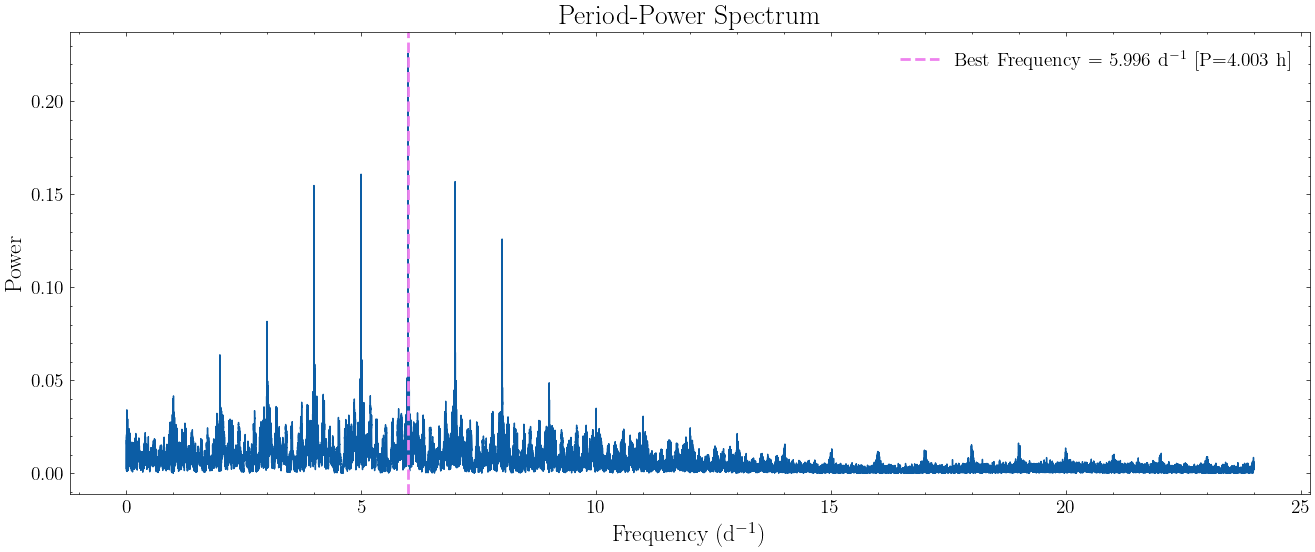
\includegraphics[scale=0.55]{Metodologia/Secciones/AnalisisPeriodo/Figures/LS Power Spectrum.png}
	
	\caption{Espectro de frecuencias de las curvas de luz fotométricas de
	\atoObjIdNoSpace, usando los datos recabados de Iturbide y de Gaia. Esta fue
	generada usando el periodograma dentro de los estimadores de PHOEBE, el cual
	utiliza el periodograma Lomb-Scargle en Astropy. El pico de más alta
	potencia está ubicado en el periodo de 0.16677069137624234 d [4.002496593
	h]} 
	\label{periodogramaLSFrecs}
\end{figure}

Dado este espectro de frecuencias encontramos que el periodo orbital yace en la
segunda armónica de la frecuencia principal. Esto se debe a los requisitos para
analizar una curva de luz de un sistema binario eclipsante; estos muestran dos
valles en el espacio fase, las cuales corresponden a las etapas en la curva de
luz en las que se observan eclipses en el sistema. Esto es necesario para poder
modelar la curva de luz en fase como una Gaussiana doble, el modelo aceptado
para una binaria eclipsante. %TODO: agrega bibliografía
Utilizando la segunda armónica de la frecuencia de más alta potencia se puede
ver esta forma esperada de la curva de luz, como se puede ver en la figura
\ref{gaiaIturbidePhaseFold}. El periodo orbital encontrado es de 8.0049931 horas.

\begin{figure}[!h]
	\centering
	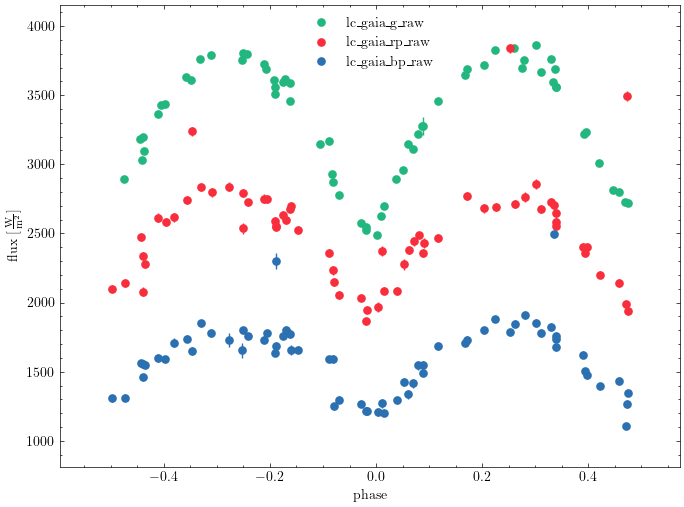
\includegraphics[scale=0.72]{Metodologia/Secciones/AnalisisPeriodo/Figures/Gaia Phase-Folded.png}
	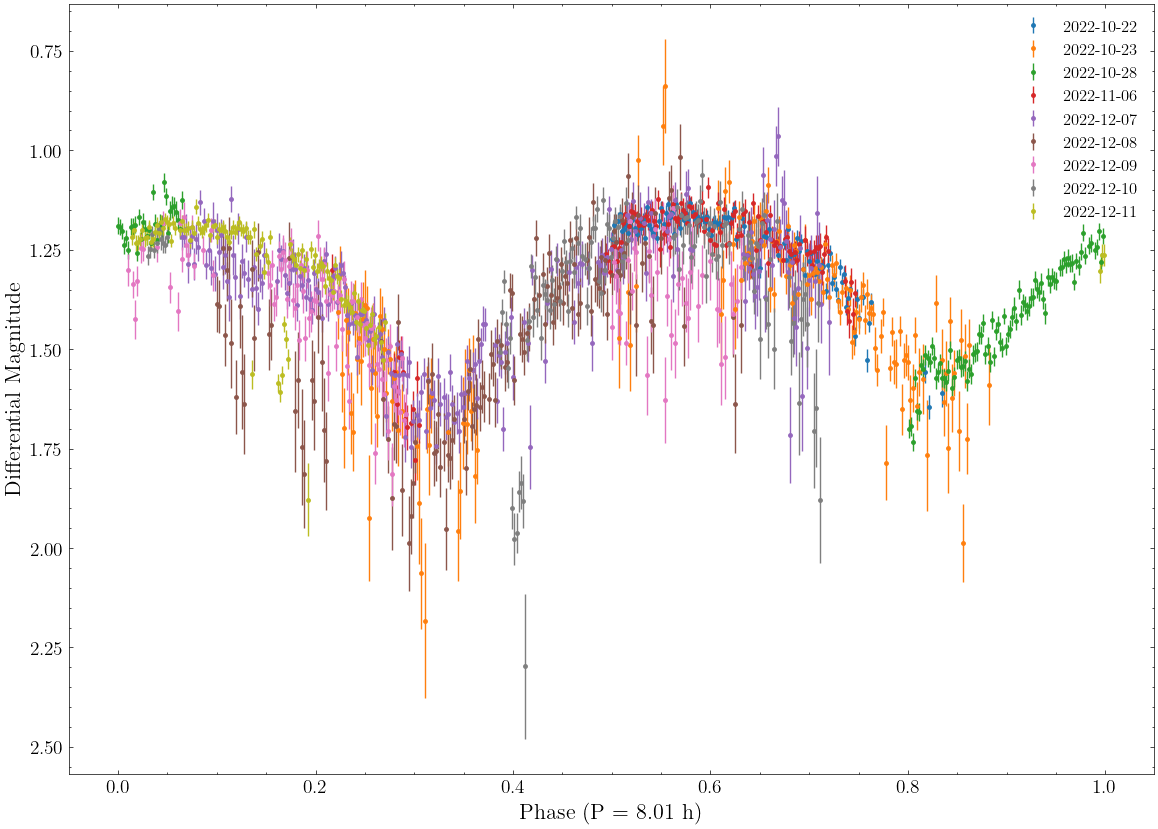
\includegraphics[scale=0.72]{Metodologia/Secciones/AnalisisPeriodo/Figures/Iturbide Phase-Folded.png}

	\caption{Curvas de luz de Gaia e Iturbide en espacio fase dado un periodo
		orbital de 8.0049 horas. En este momento las curvas de luz de Gaia
		muestran un comportamiento desordenado debido a que el tiempo de
		conjunción superior del sistema no ha sido bien definido, y actualmente
		se encuentra en su valor inicial de $0.0$, el cual no es correcto para
		este sistema. Tanto el periodo orbital como el tiempo de conjunción
		superior son corregidos en los siguientes pasos de afinación del modelo
		de PHOEBE.}
	\label{gaiaIturbidePhaseFold}
\end{figure}